
%(BEGIN_QUESTION)
% Copyright 2010, Tony R. Kuphaldt, released under the Creative Commons Attribution License (v 1.0)
% This means you may do almost anything with this work of mine, so long as you give me proper credit

Suppose we have an Allen-Bradley SLC 500 PLC with a water level switch and a temperature switch we need to connect to it:

$$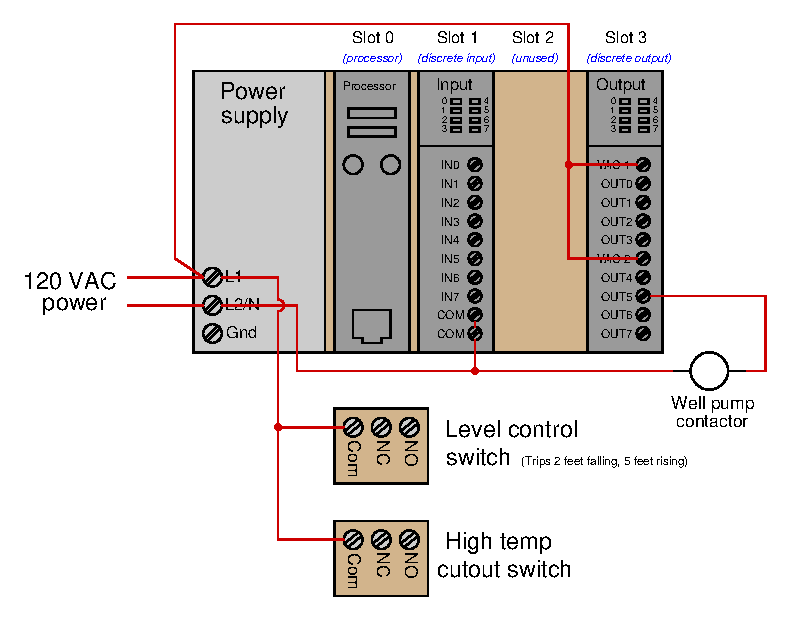
\includegraphics[width=15.5cm]{i02253x01.eps}$$

The purpose of this PLC control is to start and stop a water pump drawing water from a well, to maintain a minimum water level in a storage tank.  The level switch measures the water level in the storage tank to control the pump.  The problem is, the pump will overheat if run continuously, so a high-temperature ``cutout'' switch is installed at the motor to sense motor temperature and shut off the pump if the motor gets too hot.  The PLC will immediately shut off the motor if it senses a high temperature, and refuse to re-start the motor for at least 5 minutes after the temperature has fallen below the temperature switch's trip point.

\filbreak

Someone else has already written the program for this PLC, leaving you to figure out which contact on each switch (NO or NC) must be connected to which terminal on the input card.  Sketch wires for all connections to complete this system, based on this pre-written Ladder Diagram program:

$$\includegraphics[width=15.5cm]{i02253x02.eps}$$

\vfil 

\underbar{file i02253}
\eject
%(END_QUESTION)





%(BEGIN_ANSWER)

This is a graded question -- no answers or hints given!

%(END_ANSWER)





%(BEGIN_NOTES)

According to the verbal description of this system's operation, the temperature switch is associated with the 5 minute ``lockout'' timer function.  Therefore, input {\tt I:1/4} must be the one connected to the temperature switch.  From the PLC program shown we see that this input controls an off-delay timer (TOF), which in turn enables or disables output {\tt O:3/5} which controls the pump motor.

When the motor is cool, we want the program to enable it to run.  This means we need to have the {\tt T4:1/DN} contact instruction colored (able to pass virtual power to the output coil instruction {\tt O:3/5}).  Seeing as the {\tt T4:1/DN} instruction is normally-closed, this means we need the timer's ``done'' bit to be in a zero state during regular operation, which means the timer instruction's input needs to be ``false'' (i.e. no color on the {\tt I:1/4} contact instruction).  Seeing as the {\tt I:1/4} contact is normally-closed, this means we need the {\tt I:1/4} bit to be in a 1 state when the motor is cool, in order to maintain that contact instruction in its un-colored state and not activate the timer.  This in turn means that input channel IN4 needs to be powered when the motor is cool, necessitating the use of normally-closed contacts on the temperature switch.

\vskip 10pt

The water level switch, sensing level inside the storage tank, needs to turn the well pump motor on when level inside the tank is too low.  Looking at the PLC program we see that the only other input {\tt I:1/0} is associated with a normally-open instruction on the rung sending virtual power to output coil {\tt O:3/5}.  Since activating this coil instruction is what starts up the pump motor, we need the contact instruction {\tt I:1/0} to be colored when the pump needs to run.  This means we need to have input bit {\tt I:1/0} set to a ``1'' state when the pump needs to run.  The pump needs to run whenever tank level is low, and so we need the level switch to send power in PLC input channel IN0 when it senses a low liquid level (i.e. its ``normal'' state according to the switch manufacturer), and so we must wire the liquid level switch to use its normally-closed (NC) contacts.

$$\includegraphics[width=15.5cm]{i02253x03.eps}$$

%INDEX% PLC, relating I/O status to virtual elements 

%(END_NOTES)


